\renewcommand{\thesection}{\arabic{section}}\renewcommand{\theHsection}{chapter.\arabic{section}}\setcounter{section}{0}\section{运动方程}
\noindent\begin{minipage}{\textwidth}\ProblemHeading{例题}{1.1（改写）}
分别考虑行星绕太阳公转和行星绕自身轴线自转。判断在描述哪一种运动时可以把行星视为质点，并说明理由。
\end{minipage}\par\vfill
\noindent\begin{minipage}{\textwidth}\ProblemHeading{例题}{1.2（改写）}
一个不受外力的物体在某时刻相对于所选参考系速度为零。分别在所选参考系为惯性系和为非惯性系的情况下，判断物体此后是否必定相对于该参考系保持静止，并说明理由。
\end{minipage}\par\vfill
\newpage
\noindent\begin{minipage}{\textwidth}\ProblemHeading{例题}{1.3（改写）}
在惯性参考系中，考虑一个自由质点。由空间和时间的均匀性及空间的各向同性，可取其拉格朗日函数为 $L=f(v^2)$。设伽利略变换令速度由 $\mathbf v$ 变为 $\mathbf v+\mathbf V$。
\SubQ{1}{利用无穷小的恒定速度 $\mathbf V$，以及变换前的 $L$ 与变换后的 $L$ 至多相差一个关于坐标和时间的函数对时间的全导数，确定 $f(v^2)$ 的形式。}
\SubQ{2}{对任意恒定的 $\mathbf V$，把变换前后拉格朗日函数的差显式写成对时间的全导数。}
\end{minipage}\par\vfill
\noindent\begin{minipage}{\textwidth}\ProblemHeading{例题}{1.4（改写）}
在惯性参考系中，质量为 $m$ 的自由质点的拉格朗日函数为 $L=mv^2/2$。求下列坐标系中的弧长微元平方 $\mathrm dl^2$，并分别写出 $L$。
\SubQ{1}{笛卡儿坐标 $(x,y,z)$。}
\SubQ{2}{柱坐标 $(r,\varphi,z)$，其中 $r$ 为到 $z$ 轴的距离，$\varphi$ 为方位角。}
\SubQ{3}{球坐标 $(r,\theta,\varphi)$，其中 $r$ 为到原点的距离，$\theta$ 为与 $z$ 轴正向的夹角，$\varphi$ 为方位角。}
\end{minipage}\par\vfill
\newpage
\noindent\begin{minipage}{\textwidth}\ProblemHeading{习题}{1.5}
如图，平面双摆由质量分别为 $m_1$、$m_2$ 的两个质点和长度分别为 $l_1$、$l_2$ 的两根轻绳组成。两绳与竖直向下方向的夹角分别为 $\varphi_1$、$\varphi_2$。在重力加速度为 $g$ 的均匀重力场中，求该系统的拉格朗日函数。
\begin{center}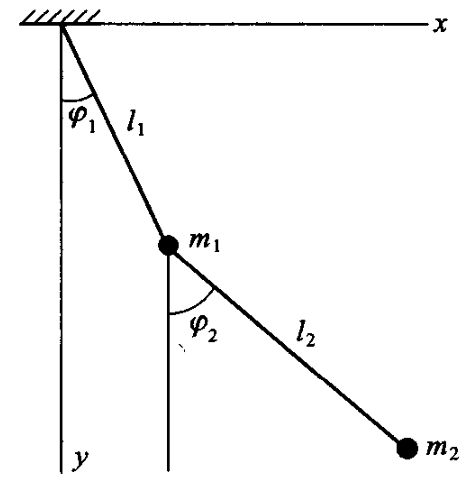
\includegraphics[width=0.28\linewidth]{figures/fig_1_5_1.png}\end{center}
\end{minipage}\par\vfill
\noindent\begin{minipage}{\textwidth}\ProblemHeading{习题}{1.6}
一平面摆的摆球质量为 $m_2$，悬挂点质量为 $m_1$，可沿水平直线运动。摆长为 $l$，坐标如图。在重力加速度为 $g$ 的均匀重力场中，求该系统的拉格朗日函数。
\begin{center}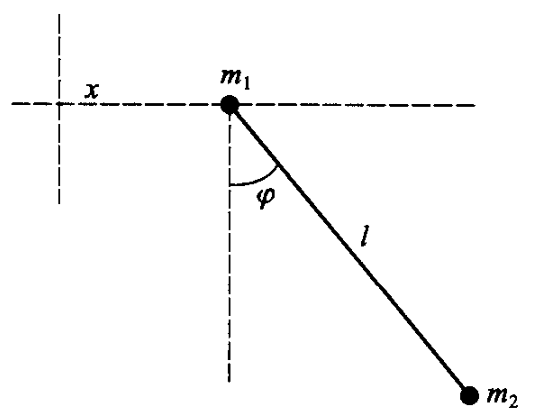
\includegraphics[width=0.28\linewidth]{figures/fig_1_6_1.png}\end{center}
\end{minipage}\par\vfill
\newpage
\noindent\begin{minipage}{\textwidth}\ProblemHeading{习题}{1.7}
一平面摆的摆球质量为 $m$，摆长为 $l$。设均匀重力场的重力加速度为 $g$。求下列各情形中平面摆的拉格朗日函数。
\SubQ{1}{悬挂点沿半径为 $a$ 的竖直圆以恒定角频率 $\gamma$ 运动，如图所示。}
\SubQ{2}{悬挂点沿水平方向振动，位移为 $a\cos\gamma t$。}
\SubQ{3}{悬挂点沿竖直方向振动，位移为 $a\cos\gamma t$。}
\begin{center}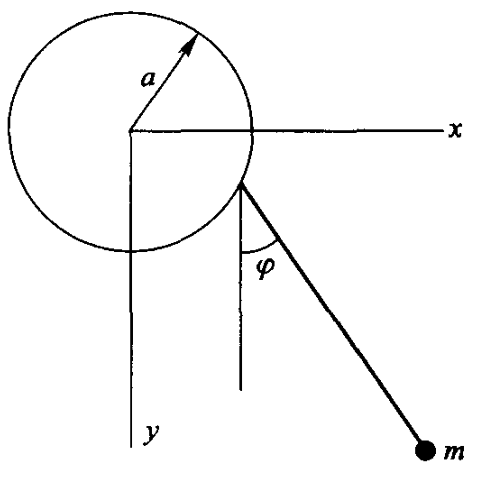
\includegraphics[width=0.28\linewidth]{figures/fig_1_7_1.png}\end{center}
\end{minipage}\par\vfill
\noindent\begin{minipage}{\textwidth}\ProblemHeading{习题}{1.8}
如图，四根长度均为 $a$ 的轻杆铰接成菱形，顶端 $A$ 固定，左右两端各有一个质量为 $m_1$ 的质点，底端质量为 $m_2$ 的质点沿竖直轴运动。整个系统以恒定角速度 $\Omega$ 绕该轴转动。设均匀重力场的重力加速度为 $g$，求该系统的拉格朗日函数。
\begin{center}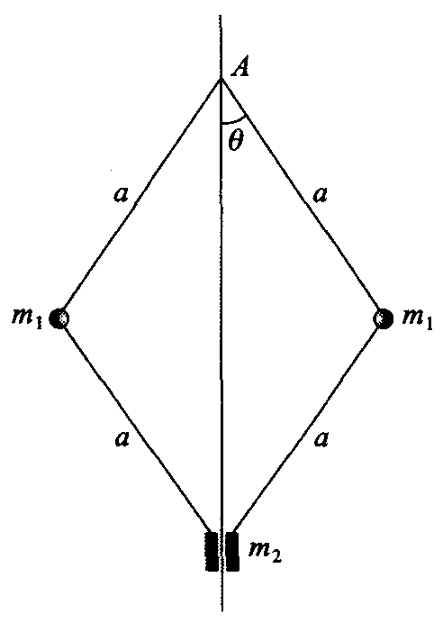
\includegraphics[width=0.24\linewidth]{figures/fig_1_8_1.png}\end{center}
\end{minipage}\par\vfill
